\documentclass[10pt]{article}

\usepackage{parskip}
\usepackage[margin=1in]{geometry} 
\usepackage{amsmath,amsthm,amssymb, graphicx, multicol, array}
\usepackage[style=apa]{biblatex}
\addbibresource{sources.bib}
\usepackage{enumitem}
\usepackage{tikz}
\usepackage{booktabs}
\usepackage{footmisc}
\usepackage{amssymb}
\usepackage{float}
\usepackage{href-ul}
 
\newcommand{\N}{\mathbb{N}}
\newcommand{\Z}{\mathbb{Z}}
 
\newenvironment{problem}[2][Problem]{\begin{trivlist}
\item[\hskip \labelsep {\bfseries #1}\hskip \labelsep {\bfseries #2.}]}{\end{trivlist}}

\begin{document}
 
\title{Assignment 2 \\Macro Theory}
\author{Jakob Sverre Alexandersen\\
GRA4159 Trends, Cycles \& Signals Extraction}
\maketitle

Despite your young age and lack of experience you have been appointed as governor of the
Norwegian central bank (Norges Bank). However, you enter the stage at a difficult time. The
Covid-19 pandemic disrupted global supply chains and inflation has been above target for a
long time period. Moreover, it is war in Europe and political unrest, which all potentially have
adverse effects on demand.

Against this background, a journalist wants to write an article about Norges Bank's interest
rate considerations. The journalist has gotten an interview appointment with you (serving as
governor of the Norwegian central bank!)

\begin{enumerate}
    \item Use your understanding of RS (on the curriculum) to discuss the potential arguments for
    and against lowering the interest rate given today's macroeconomic situation

    The journalist is a very quantitative person writing for a quantitative magazine. Thus, it is
    expected that you use equations and diagrams --- as in RS --- in your argumentation. Your
    answer should be roughly 1 page of text, excluding equations and diagrams.
\end{enumerate}

More generally:

    \begin{enumerate}[resume]
    \item In RS (on the curriculum) it is stated that: “Many central banks abandoned fixed
    exchange rates in favor of flexible inflation targeting to stabilize the domestic economy
    more directly.” Discuss shortly what the term “fixed exchange rate” means in this
    context.
    \item Given your knowledge of RS, discuss shortly to what extent the central bank can control
    the trend component of GDP.
\end{enumerate}

Unfortunately, it is not only the short- and medium-term macroeconomic developments that
are worrying. In fact, for a long time there has been much academic and policy debate about
the negative productivity developments in many western economies, including Norway.

Last year, the former industry leader Martin Bech Holte wrote a bestselling book about the
issue, titled The Country That Became Too Rich. This autumn (2025) he came with a follow-up
that created a lot of controversy as well --– as exemplified by this commentary written by
Terje Erikstad in \href{https://www.dn.no/kommentar/martin-bech-holte/produktivitet/produktivitetsvekst/martin-bech-holte-bor-trekke-boken-alternativt-statsbudsjett/2-1-1917021}{Dagens Næringsliv}

Read about how do growth accounting using the so-called neoclassical production function in
the slide deck titled “tfpProductionFunction.pdf”. Next read the two first chapters in the
research article titled “Review of Income and Wealth - 2024 - Fernald - The Productivity
Slowdown.pdf” --- both available on Itslearning. Then:

\begin{enumerate}[resume]
    \item Write half-a-page clarifying the relationship between growth regressions, as defined in
    the World Bank report in Assignment 1, and the growth accounting framework described
    in the documents referred to above. Clarify, in particular:
    \begin{enumerate}
        \item Overall similarity and differences between the two approaches
        \item Whether such regressions or decompositions are causal
    \end{enumerate}
    \newpage 
    \item Use the national account statistics produced by SSB to collect time series on annual
    \begin{enumerate}
        \item Real GDP for Mainland Norway
        \item The capital stock in real terms
        \item Hours worked
        \item Wage costs and production in nominal terms
    \end{enumerate}
\end{enumerate}
\newpage 
\section{Divine Coincidence or Dangerous Trade-off?}
\cite{roisland_sveen_2018_monetary_policy_inflation_targeting} (RS) present a model where the central bank aims to stabilize both inflation and output. The economy is described by two fundamental relationships. First, aggregate demand follows an IS curve:
\begin{gather*}
    y = -\alpha(r - \bar{r})
\end{gather*}
where $y $ is the output gap (actual output relative to potential), $r $ is the real interest rate, and $\bar{r} $ is the neutral real rate that would close the output gap. When the real interest rate exceeds the neutral rate, demand falls and the economy enters recession. When it is below, the economy booms. 

Second, the supply side is captured by a Phillips curve relating inflation to economic activity: 
\begin{gather*}
    \pi = \pi^e + \gamma y + u
\end{gather*}
Here inflation $\pi $ depends on expected inflation $\pi^e $, the output gap (through the coefficient $\gamma $), and a cost-push shock $u $ representing factors like energy price surprises or unexpected wage developments.

The central bank's objective is formalized through a loss function: 
\begin{gather*}
    L = \frac{1}{2}\left[(\pi - \pi^*)^2 + \lambda y^2\right]
\end{gather*}
This captures that the central bank dislikes both deviations of inflation from target $\pi^* $ and deviations of output from potential. The parameter $\lambda $ reflects the relative weight placed on output stability, which is what distinguishes ``flexible'' from ``strict'' inflation targeting.

Minimizing this loss function subject to the economic constraints yields an optimality condition: 
\begin{gather*}
    \pi - \pi^* = -\frac{\lambda}{\gamma}y
\end{gather*}
This relationship states that either both gaps are zero (the ideal outcome), or they must have opposite signs. If inflation is above target, output should be below potential, and vice versa. The central bank can never be in an optimal position if both gaps are positive or both negative simultaneously.

\subsection{Arguments for Lowering Interest Rates}

Current political unrest and war in Europe are conditions that could (and have) dampen demand. If we interpret this as a negative demand shock, the RS framework provides clear guidance. In a closed economy, demand shocks create what the literature calls ``divine coincidence'' (\cite{87e157cf-0c39-3c03-80d6-6ece5bed6979}); there is no conflict between stabilizing inflation and stabilizing output. 

Figure~\ref{fig:demand} illustrates this case. A negative demand shock shifts the IS curve leftward from $IS$ to $IS'$. At the original interest rate $\rho$, output falls to $y'$ and inflation drops to $\pi'$, both of which fall below target. Since both gaps are negative, the optimality condition is violated. The central bank can restore equilibrium by cutting rates to $r''$, shifting IS back and returning both output and inflation to their target levels. This is the divine coincidence: stabilizing output automatically stabilizes inflation.

This logic suggests that if Norwegian policymakers are primarily worried about weak demand from geopolitical uncertainty, interest rate cuts would be warranted. A reduction in $r$ stimulates demand through the IS relationship, which in turn puts upward pressure on inflation through the Phillips curve, addressing both concerns at once.

\begin{figure}[H]
\centering
    \begin{tikzpicture}[scale=1.1]
    
    % ================= TOP PANEL =================
    \draw[->] (0,0) -- (7,0) node[right] {$y$};
    \draw[->] (0,0) -- (0,4) node[above] {$\pi$};
    
    \draw[thick] (0.8,3.5) -- (6.2,0.8) node[right] {$MP$};
    \draw[thick] (0.8,0.8) -- (6.2,3.5) node[right] {$PC$};
    
    \coordinate (E) at (3.5,2.1);
    
    % Dotted guides through intersection
    \draw[dotted] (E) -- (E |- 0,0);
    \draw[dotted] (0,2.1) -- (E);
    
    % pi' guides
    \draw[dotted] (0,1.7) -- (2.4,1.7);
    \draw[dotted] (2.4,0) -- (2.4,1.7);
    
    % Labels
    \node[left]  at (0,2.1) {$\pi^*$};
    \node[left]  at (0,1.7) {$\pi'$};
    \node[below] at (2.4,0) {$y'$};
    
    % ================= BOTTOM PANEL =================
    \begin{scope}[yshift=-5cm]
    
    \draw[->] (0,0) -- (7,0) node[right] {$y$};
    \draw[->] (0,0) -- (0,4) node[above] {$r$};
    
    \draw[thick] (0.8,3.3) -- (6.2,0.9) node[right] {$IS$};
    \draw[thick] (0.8,2.7) -- (6.2,0.3) node[right] {$IS'$};
    
    \draw[dotted] (2.4,0) -- (2.4,4);
    \draw[dotted] (3.5,0) -- (3.5,4);
    
    \draw[dotted] (0,2.2) -- (3.5,2.2);
    \draw[dotted] (0,1.6) -- (3.5,1.6);
    
    \node[left]  at (0,2.2) {$\rho$};
    \node[left]  at (0,1.6) {$r''$};
    \node[below] at (2.4,0) {$y'$};
    \node[below] at (3.5,0) {$0$};
    
    \end{scope}
    \end{tikzpicture}
\caption{Negative demand shock: divine coincidence allows full stabilization}
\label{fig:demand}
\end{figure}

\subsection{Arguments Against Lowering Interest Rates}

However, inflation has been above target for an extended period. This represents a positive cost-push shock $(u > 0)$ in the Phillips curve. Unlike demand shocks, cost-push shocks create a genuine policy trade-off, the divine coincidence breaks down. 

Figure~\ref{fig:costpush} illustrates this case. When $u > 0$, the Phillips curve shifts upward from $PC$ to $PC'$. At the original equilibrium where $y = 0$, inflation would now be at $\pi'$, above the target $\pi^*$. This violates the optimality condition because the inflation gap is positive while the output gap is zero. Unlike with demand shocks, the central bank cannot restore both gaps to zero simultaneously.

The optimal response, shown at point $B$, requires the central bank to raise interest rates, engineering a negative output gap $y'$ to partially bring inflation down toward $\pi''$. The central bank must accept some deviation in both variables --- this is the policy trade-off. With flexible inflation targeting $(\lambda > 0)$, the central bank tolerates some above-target inflation rather than forcing output far below potential.

Norway is also an open economy, where lower rates cause the NOK to depreciate, directly raising import prices through the ``direct exchange rate channel''. This means even demand shocks cannot be perfectly neutralized; cutting rates weakens the currency and pushes inflation higher.

\begin{figure}[H]
\centering
    \begin{tikzpicture}[scale=1.1]
    
    % ================= TOP PANEL =================
    \draw[->] (0,0) -- (7,0) node[right] {$y$};
    \draw[->] (0,0) -- (0,4) node[above] {$\pi$};
    
    % MP curve (downward sloping)
    \draw[thick] (0.8,3.5) -- (6.2,0.8) node[right] {$MP$};
    
    % Original PC curve (upward sloping, through origin area)
    \draw[thick] (0.8,0.8) -- (6.2,3.5) node[right] {$PC$};
    
    % Shifted PC' curve (upward sloping, higher intercept)
    \draw[thick] (0.8,1.5) -- (6.2,4.2) node[right] {$PC'$};
    
    % Original equilibrium at y=0, pi=pi*
    \coordinate (A) at (3.5,2.15);
    
    % New equilibrium after cost-push shock (on MP curve, intersection with PC')
    \coordinate (B) at (2.6,2.55);
    
    % Point showing pi' if y stayed at 0 (on PC' where y=0)
    \coordinate (C) at (3.5,2.85);
    
    % Dotted guides for original equilibrium
    \draw[dotted] (3.5,0) -- (3.5,2.85);
    \draw[dotted] (0,2.15) -- (A);
    
    % Dotted guides for new equilibrium B
    \draw[dotted] (0,2.55) -- (B);
    \draw[dotted] (2.6,0) -- (2.6,2.55);
    
    % Dotted guide for pi' (inflation if no response)
    \draw[dotted] (0,2.85) -- (C);
    
    % Labels
    \node[left]  at (0,2.15) {$\pi^*$};
    \node[left]  at (0,2.55) {$\pi''$};
    \node[left]  at (0,2.85) {$\pi'$};
    \node[below] at (3.5,0) {$0$};
    \node[below] at (2.6,0) {$y'$};
    
    % Point labels
    \fill (A) circle (2pt) node[above right] {$A$};
    \fill (B) circle (2pt) node[above left] {$B$};
    
    % ================= BOTTOM PANEL =================
    \begin{scope}[yshift=-5cm]
    
    \draw[->] (0,0) -- (7,0) node[right] {$y$};
    \draw[->] (0,0) -- (0,4) node[above] {$r$};
    
    % IS curve (unchanged - cost-push doesn't shift IS)
    \draw[thick] (0.8,3.3) -- (6.2,0.9) node[right] {$IS$};
    
    % Dotted guides
    \draw[dotted] (2.6,0) -- (2.6,4);
    \draw[dotted] (3.5,0) -- (3.5,4);
    
    \draw[dotted] (0,2.2) -- (3.5,2.2);
    \draw[dotted] (0,2.6) -- (2.6,2.6);
    
    \node[left]  at (0,2.2) {$\rho$};
    \node[left]  at (0,2.6) {$r'$};
    \node[below] at (2.6,0) {$y'$};
    \node[below] at (3.5,0) {$0$};
    
    \end{scope}
    \end{tikzpicture}
\caption{Cost-push shock: the policy trade-off}
\label{fig:costpush}
\end{figure}

\subsection{Conclusion}

Given that Norwegian inflation currently stands around 3 percent, above the 2 percent target, and stems largely from supply-side factors, the RS framework suggests caution. The cost-push nature of current inflation means there is no free lunch. The central bank must choose between tolerating above-target inflation or accepting below-potential output. This explains Norges Bank's gradual approach rather than aggressive cuts.

\section{Fixed Exchange Rate}
In RS, ``fixed exchange rate'' refers to a regime where the CB commits to keeping the domestic currency at a chosen level against another currency, or a basket of currencies. The main policy objective is to stabilize the exchange rate, not domestic inflation or output. 

When RS say that many central banks have ``abandoned fixed exchange rates in favor of flexible inflation targeting to stabilize the domestic economy more directly,'' they mean that by giving up the exchange-rate peg and adopting a flexible exchange rate with an inflation target, the CB can use the policy rate to steer domestic inflation and real activity (the output gap) directly, instead of subordinating monetary policy to the exchange-rate objective.
\newpage 
\section{Control of the Trend Component}
The central bank cannot control the trend component of GDP. RS state that monetary policy has only temporary effects on the real economy and is neutral in the long run. In the long run, output is determined by technology, preferences, and access to factors of production, i.e., by real (supply-side) factors, not by the policy rate itself. What monetary policy can do is stabilize demand around potential output: it can influence the output gap, not the level or growth rate of potential output itself. The loss function in RS is defined in terms of the inflation gap and the output gap; the central bank is assumed to care about stabilizing output around potential, not about raising potential. Structural unemployment and long-run output are taken as given by labor-market and supply-side conditions. 

In short, the CB can affect the cyclical component of GDP (the gap around trend), but not the trend itself. That is determined by real factors outside the scope of monetary policy. 
\section{Relationship Between Growth Regressions and Growth Accounting}
Growth regressions, as in the World Bank report (\cite{wacker2024leveraging}), model (log) income or growth as a function of ``growth correlates'', e.g., infrastructure, human capital, trade, and macro policy, in a panel or cross-section of countries. They deliver partial correlations: how much growth (or income) is associated with each variable, holding others constant. The report stresses that these regressions are useful for comparative country analysis and for assessing how ``typical'' a country's growth pattern is, but that least-squares estimates are ``estimated partial correlations rather than causal effects'' (\cite[p. 3]{wacker2024leveraging}), due to endogeneity such as omitted variables and reverse causality. 

Growth accounting, as in the ``tfpProductionFunction'' deck and \cite{fernald_inklaar_ruzic_2025_productivity_slowdown}, starts from the Cobb-Douglas production function $Y_t = A_t K_t^\alpha L_t^{1-\alpha}$ and decomposes output growth into contributions from growth in capital, growth in labor, and a residual (TFP). So it allocates observed growth to factor accumulation and to ``everything else'', rather than regressing growth on many correlates. 

The two approaches are similar in that both aim to describe what is associated with growth, both are motivated by the neoclassical framework, and both provide a form of attribution; growth accounting to $K, L$, and TFP, and growth regressions to policy-relevant variables. The differences are that growth accounting is mechanical decomposition, and growth regressions are multivariate regressions. In addition, growth accounting answers ``how much of this country's growth came from capital, labor, and TFP?''; growth regressions answer ``how is growth correlated with infrastructure, education, trade, etc. across countries?'' Growth accounting typically uses national-accounts data country by country, and growth regressions use a broad set of correlates and income/growth across many countries.

In terms of causality, neither approach is causal. The World Bank report states that growth-regression estimates are partial correlations, not causal effects, because of endogeneity. Growth accounting is an accounting decomposition: it attributes observed growth to factors and a residual. It does not claim that, say, ``capital accumulation caused this much growth'' in a causal sense. For causal claims, one would need identification strategies, as the report also notes. 
\newpage 
\section{Plots}
\subsection{Real GDP for Mainland Norway}
\begin{figure}[H]
    \centering
    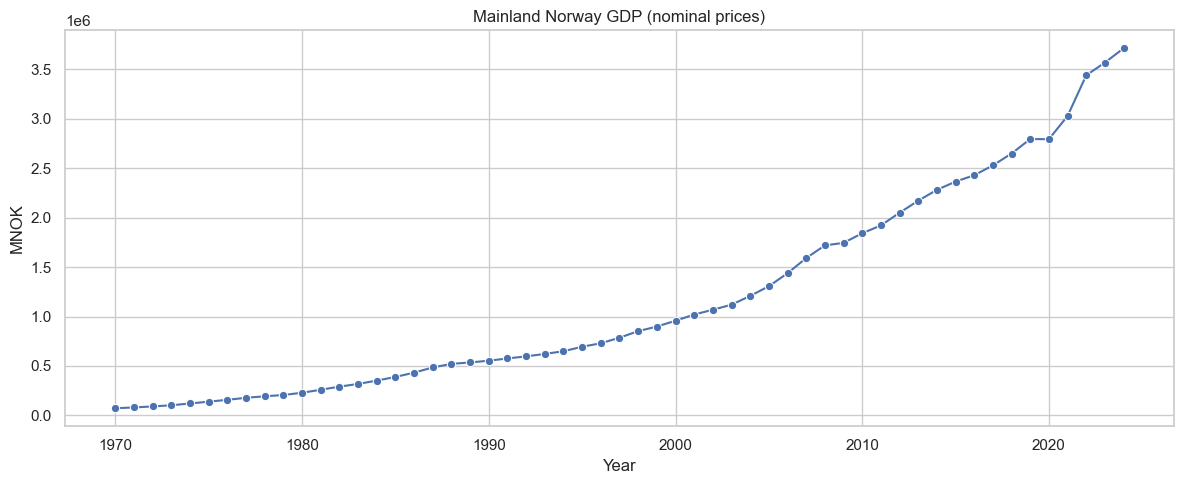
\includegraphics[width=1\textwidth]{2026-02-06-10-16-41.png}
\end{figure}
\subsection{The capital stock in real terms}
\begin{figure}[H]
    \centering
    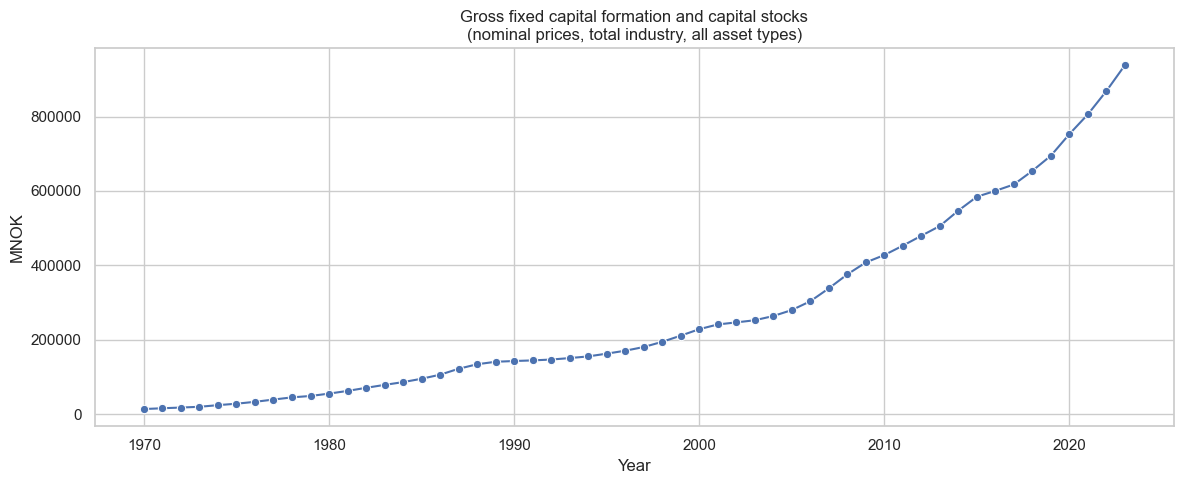
\includegraphics[width=1\textwidth]{2026-02-06-10-19-10.png}
\end{figure}
\newpage 
\subsection{Hours Worked (for employees -- self-employed excluded)}
\begin{figure}[H]
    \centering
    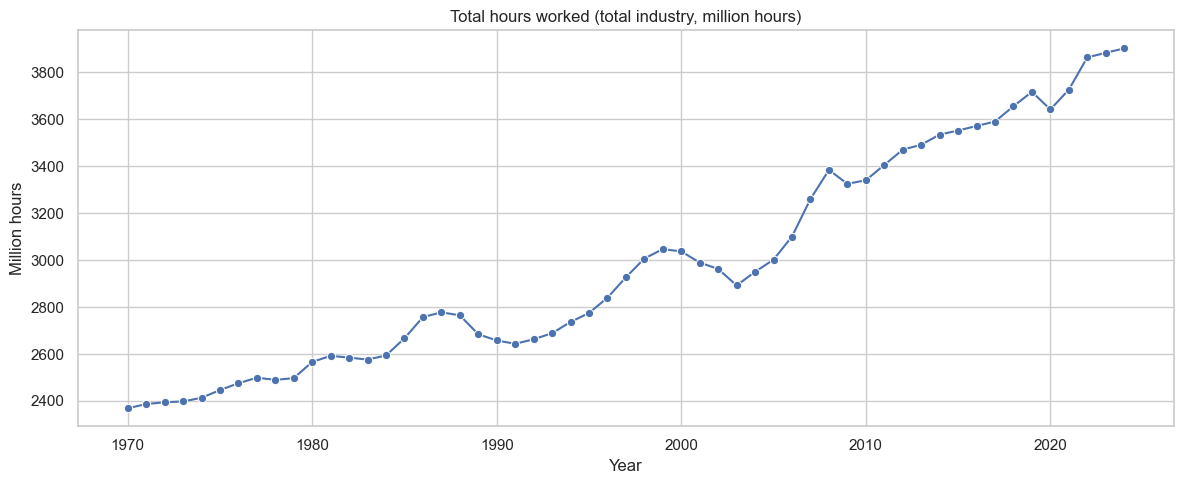
\includegraphics[width=1\textwidth]{2026-02-06-10-03-53.png}
\end{figure}
\subsection{Wage costs and production in nominal terms}
\begin{figure}[H]
    \centering
    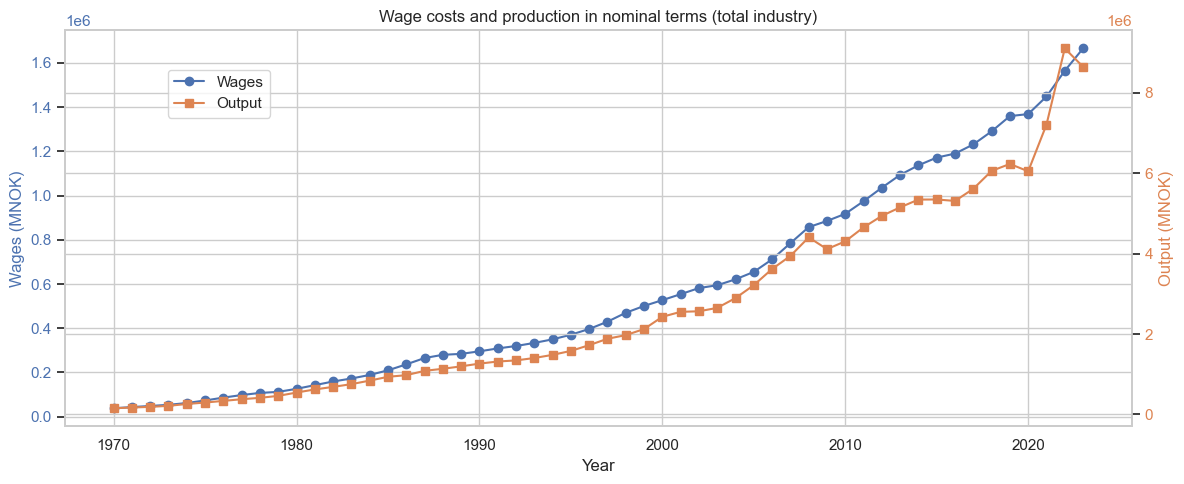
\includegraphics[width=1\textwidth]{2026-02-06-10-40-45.png}
\end{figure}
\newpage 
\printbibliography

\end{document}